\documentclass[apectratio=169]{beamer}
\usetheme{metropolis}           % Use metropolis theme
% For PDFs
\usepackage{pdfpages}
\usepackage{minted}
\usepackage{tabularx}
\title{Swakeup}
\subtitle{More Than A Simple Wakeup Light}
\date{\today}
\author{Elmar van Rijnswou and Maximilian Stiefel}
\institute{Uppsala University}
\begin{document}
  \maketitle

\begin{frame}{Table Of Contents}
  \setbeamertemplate{section in toc}[sections numbered]
  \tableofcontents[hideallsubsections]
\end{frame}

  \section{Introduction}
  	\begin{frame}{Poka-yoke}
		\only<1>{\Large Who knows what Poka-yoke is?}
		\only<2>{
		\metroset{block=fill}
		\begin{block}{Poka-yoke (Wikipedia)}
		Poka-yoke [poka joke] is a Japanese term that means
		"mistake-proofing" or “inadvertent error prevention”.
		\end{block}
		}
	\end{frame}
	\begin{frame}{Background}
		\begin{figure}
        		\centering
                	\includegraphics[width=1\textwidth]{./fig/darkness}
			\caption{According to Sveriges Radio ”many Swedes suffer
		from the winter blues or seasonal affective disorder”.
		Image Source: Visitsweden}
		\end{figure}
	\end{frame}

  	\begin{frame}{System Requirements}
		\begin{itemize}
			\item<1-> Wakeup light which is a part of the \textit{IoT}
			\item<2-> Swakeup \ensuremath{\rightarrow} engl. "Swedish Wakeup Light"
			\item<3-> Wakes up, displays time, weather, mails, facebook
			\item<4-> Smart, small, USB charger included
			\item<5-> Spends happiness
		\end{itemize}
  	\end{frame}
  	\begin{frame}{System Overview}	
		\begin{figure}
			\centering
			\only<2>{\includegraphics[height=0.8\textheight]{../block/block.png}}
			\only<1>{\includegraphics[height=0.6\textheight]{../block/block_simplified.png}}
			\caption{System Overview}
		\end{figure}
	\end{frame}
  
  \section{Hardware}
  	\begin{frame}{Power Board}
		\begin{figure}
			\centering
			\only<1>{\includegraphics[width=0.95\textwidth]{./fig/power1}}
			\only<2>{\includegraphics[width=0.95\textwidth]{./fig/power2}}
			\only<3>{\includegraphics[width=0.95\textwidth]{./fig/power3}}



			\caption{Power Board Schematics}
		\end{figure}	
  	\end{frame}
  	\begin{frame}{Logic Board}	
		\begin{figure}
			\centering
			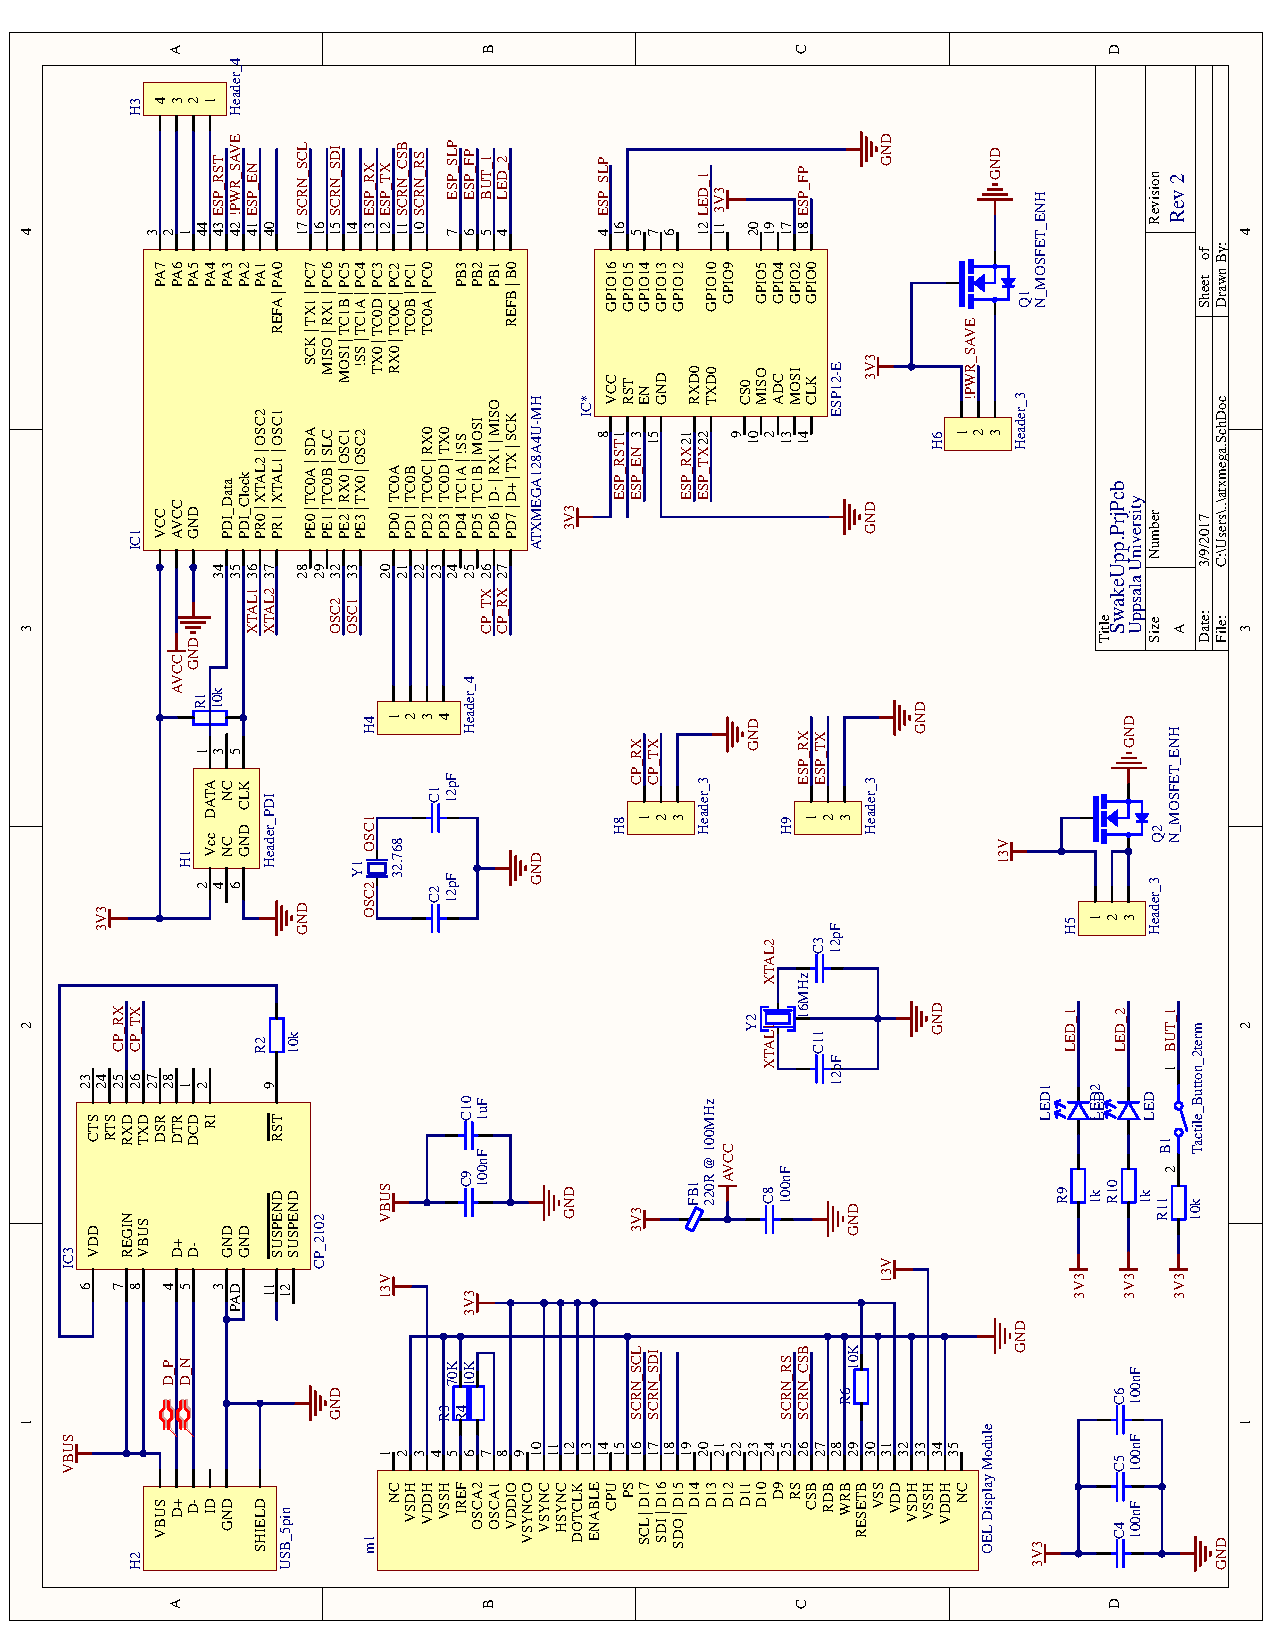
\includegraphics[height=0.8\textheight]{./fig/logic}
			\caption{Logic Board Schematics}
		\end{figure}
	\end{frame}

  \section{Software}
  	\begin{frame}{Code Structure}
		 \begin{figure}
                        \centering
                        \includegraphics[width=0.6\textwidth]{./fig/code_structure}
                        \caption{Abstract Layering Model}
                \end{figure}
  	\end{frame}
	\begin{frame}{Code Organisation}
		 \begin{figure}
                        \centering
                        \includegraphics[width=0.5\textwidth]{./fig/block_code}
                        \caption{Block Diagram Of The Code Organisation}
                \end{figure}
  	\end{frame}

\begin{frame}[fragile]{Operating System - Modules And Events}
\begin{minted}[baselinestretch=1, fontsize=\tiny, linenos,frame=single,framesep=5pt]{C}
#define MODULE_DEFINE(VAR, DESC, INIT, DEINIT, ...)     \
        Module VAR = {                                  \
                .init = INIT,                           \
                .deinit = DEINIT,                       \
                .cnt = 0,                               \
                .name = DESC,                           \
                .deps = { __VA_ARGS__ }                 \
        }
MODULE_DEFINE(CORE, "Central core", init, deinit, &TIME, &COMMAND, &ESP8266);
\end{minted}

\begin{minted}[baselinestretch=1, fontsize=\tiny, linenos,frame=single,framesep=5pt]{C}
#define EVENT_REGISTER(eventName, desc)\
        Event eventName = \
        {.eventId = __COUNTER__, .data = 0, .description = desc, .descLen = sizeof(desc) }
EVENT_REGISTER(EVENT_UART_DELIMITER, "Got UART delimiter");
\end{minted}

\begin{minted}[baselinestretch=1, fontsize=\tiny, linenos,frame=single,framesep=5pt]{C}
event_addListener(&EVENT_UART_DELIMITER, callback);
\end{minted}

\begin{minted}[baselinestretch=1, fontsize=\tiny, linenos,frame=single,framesep=5pt]{C}
event_fire(&EVENT_UART_DELIMITER, SYSTEM_ADDRESS_CAST (&delimiters[USART_ID][i]));
\end{minted}


\end{frame}	
  
	\begin{frame}{Realization (1)}
	\begin{figure}
        	\centering
                \includegraphics[width=0.6\textwidth]{./fig/screen_logger}
                \caption{Screen Logging}
        \end{figure}
	\end{frame}

	\begin{frame}{Realization (2)}
	\begin{figure}
        	\centering
                \includegraphics[width=0.6\textwidth]{./fig/clock_weather}
                \caption{Appearence Of The Clock}
        \end{figure}
	\end{frame}
	
	\begin{frame}{Realization (3)}
	\begin{figure}
        	\centering
                \includegraphics[width=0.6\textwidth]{./fig/command_usage}
                \caption{USART Command Interpreter}
        \end{figure}
	\end{frame}

\begin{frame}{Realization (4)}
	\begin{figure}
        	\centering
		\only<1>{\includegraphics[height=0.8\textheight]{./fig/website1}}
                \only<2>{\includegraphics[height=0.8\textheight]{./fig/website2}}
		\only<3>{\includegraphics[height=0.8\textheight]{./fig/website3}}
		\caption{Website: Main User Interface}
        \end{figure}
	\end{frame}
 

  \section{Status Quo and Outlook}
	\begin{frame}{Basic System Functionality is Given}
	\begin{figure}
        	\centering
                \includegraphics[width=0.8\textwidth]{./fig/demo}
                \caption{Picture of Nake HW}
        \end{figure}
	\end{frame}


	\begin{frame}{Hardware} \footnotesize \begin{table}[H] \centering
		\begin{tabularx}{\textwidth}{llX} \textbf{HW Block} &
			\textbf{Working}& \textbf{Problem} \\\hline USB Charging
			& \checkmark & \\ Screen Driver & \checkmark & \\ Screen
			Driver Feedback& \checkmark & \\ Vcc for µC & \checkmark
			& \\ ESP & \checkmark & \\ Terminal & \checkmark & \\
			LED Driver & \checkmark & \\ LED Driver Feedback & &
			Reversed inputs of the differential ampifier \\ USB DCP
			& \checkmark & \\ Reverse Polarity Protection &
		\checkmark & \\ \hline \end{tabularx} \caption{Status Quo
	Hardware} \label{tab:hw_status_quo} \end{table} \end{frame}

	\begin{frame}{Software}
	\tiny
		\begin{table}[H] \centering \begin{tabularx}{\textwidth}{llX}
			\textbf{SW Block} & \textbf{Working}& \textbf{Problem}
			\\\hline UART & \checkmark & \\ SPI & \checkmark & \\
			EPROM & \checkmark & \\ Timer & \checkmark & \\	ESP8266
			& \checkmark & \\ Terminal & \checkmark & \\ SEP525F &
			\checkmark & \\ Wifi & \checkmark & \\ Command &
			\checkmark & \\ Log & \checkmark & \\ Screen &
			\checkmark & \\ Timekeeper & \checkmark & \\ Controller
			& & \\ Core & \checkmark & \\ Weather & \checkmark & \\
			Clock & \checkmark & \\ Social & & Not implemented yet
			\\ PWM & \checkmark & \\ ADC & \checkmark & \\
			Lightcontroller & \checkmark & \\ PID & \checkmark & \\
			Advanced Light Patterns & & Debugging still ongoing\\
		Play 8 bit sounds & & Not implemented, HW missing\\ \hline
		\end{tabularx} \caption{Status Quo Software}
	\label{tab:sw_status_quo} \end{table}
	\end{frame}
	
  	\begin{frame}{Outlook}	
		\begin{itemize}
			\item<1-> HW revision 3 is under construction
			\item<2-> Different functionality shall be added
			\item<3-> Housing will be constructed
			\item<4-> Social connectivity and calendar functions will be implemented
			\item<5-> Take part in Swedish Embedded Award (Embedded
				Priset)
		\end{itemize}
	\end{frame}

  	\begin{frame}{Open Source}
        	\begin{center}
                \begin{table}[]
                        \begin{tabular}{ll}
                                E: & Elmar.Vanrijnswou.9818@student.uu.se \\
                                E: & Maximilian.Stiefel.8233@student.uu.se\\
                        \end{tabular}
                \end{table}
                \includegraphics[width=0.05\textwidth]{./fig/github} \hspace{0.1cm} \url{github.com/s3xm3x/SwakeUp}\\
        	\end{center}
        	\begin{figure}
                	\includegraphics[width=0.3\textwidth]{./fig/logo}
        	\end{figure}
  	\end{frame}


  \begin{frame}[standout]
	Happy Coding :) 
  \end{frame}
\end{document}
